\documentclass{ceurart}
% \documentclass[runningheads]{llncs}

%----CEUR style
%% One can fix some overfulls
\sloppy

%----My style
\usepackage[T1]{fontenc}
\usepackage{graphicx}
\usepackage{hyperref}
\usepackage{color}
\usepackage{setspace}
\usepackage{verbatim}
\usepackage{amsmath,amssymb}
\renewcommand\UrlFont{\color{blue}\rmfamily}
% \renewcommand{\arraystretch}{0.8}
\renewcommand{\floatpagefraction}{0.9}
\renewcommand{\textfloatsep}{2.0ex}
\renewcommand{\dbltextfloatsep}{2.0ex}
\setlength{\tabcolsep}{3pt}
\newenvironment{packed_itemize}{
\vspace*{-0.5em}
\begin{itemize}
\setlength{\partopsep}{0pt}
\setlength{\itemsep}{1pt}
\setlength{\parskip}{0pt}
\setlength{\parsep}{0pt}
}{\end{itemize}}

\begin{document}

%----CEUR style
\copyrightyear{2024}
\copyrightclause{Copyright for this paper by its authors.
  Use permitted under Creative Commons License Attribution 4.0 International (CC BY 4.0).}
\conference{The 9th Workshop on Practical Aspects of Automated Reasoning,
  July 2, 2024, Nancy, France}
\title{TPTP World Infrastructure for Non-classical Logics}

\author[1]{Alexander Steen}[%
orcid=0000-0001-8781-9462,
email=alexander.steen@uni-greifswald.de,
]
\address[1]{University of Greifswald, Germany}
\author[2]{Geoff Sutcliffe}[%
orcid=0000-0001-7116-9338,
email=geoff@cs.miami.edu
]
\address[3]{University of Miami, USA}
\begin{abstract}
The TPTP World is a well established infrastructure that supports research, 
development, and deployment of Automated Theorem Proving (ATP) systems.
The development of the TPTP World has until now focused on classical logic, while many 
real-world applications of ATP also require non-classical reasoning. 
This paper describes the latest extension of the TPTP World, providing languages, problems,
solutions, and infrastructure for non-classical logics.
These are the keys steps towards releasing TPTP v9.0.0, with normal modal logic problems.
\end{abstract}
\begin{keywords}
  TPTP World \sep
  Non-classical logic
\end{keywords}

%----LNCS stype
% \title{TPTP World Infrastructure \\ for Non-classical Logics}
% \titlerunning{The Non-classical TPTP World}
% 
% \author{Alexander Steen\inst{1}\orcidID{0000-0001-8781-9462} 
% \and
% Geoff Sutcliffe\inst{2}\orcidID{0000-0001-9120-3927}}
% \authorrunning{A. Steen, G. Sutcliffe}
% \institute{University of Greifswald, Germany \\
% \email{alexander.steen@uni-greifswald.de}
% % \url{https://www.alexandersteen.de} 
% \and
% University of Miami, USA \\
% \email{geoff@cs.miami.edu}
% % \url{https://www.cs.miami.edu/home/geoff/} 
% }

\maketitle
%--------------------------------------------------------------------------------------------------
% \begin{abstract}
% The TPTP World is a well established infrastructure that supports research, 
% development, and deployment of Automated Theorem Proving (ATP) systems.
% The development of the TPTP World has until now focused on classical logic, while many 
% real-world applications of ATP also require non-classical reasoning. 
% This paper describes the latest extension of the TPTP World, providing languages, problems,
% solutions, and infrastructure for non-classical logics.
% These are the keys steps towards releasing TPTP v9.0.0, with normal modal logic problems.
% 
% \keywords{TPTP World \and Non-classical logic.}
% \end{abstract}
%--------------------------------------------------------------------------------------------------
\section{Introduction}
\label{Introduction}

The TPTP World~\cite{Sut17} is a well established infrastructure that supports research, 
development, and deployment of Automated Theorem Proving (ATP) systems.
The TPTP World includes the TPTP problem library~\cite{Sut09}, 
the TSTP solution library~\cite{Sut10}, 
standards for writing ATP problems and reporting ATP solutions~\cite{SS+06,Sut08-KEAPPA}, 
tools and services for processing ATP problems and solutions~\cite{Sut10}, 
and it supports the CADE ATP System Competition (CASC)~\cite{Sut16}.
Various parts of the TPTP World have been deployed in a range of applications,
in both academia and industry.
The web page \href{https://www.tptp.org}{\tt www.tptp.org} provides access to all 
components.

The development of the TPTP World has until now focused on classical logic, while many 
real-world applications of ATP also require non-classical reasoning. 
These applications include artificial intelligence (e.g., knowledge representation, planning, 
multi-agent systems), philosophy (e.g., formal ethics, metaphysics), natural language semantics 
(e.g., generalized quantifiers, modalities), and computer science (e.g., software and hardware 
verification).
This paper describes the latest extension of the TPTP World, providing languages and
infrastructure for reasoning in non-classical logics~\cite{Pri08,Gob01}.
The non-classical logics supported so far are
normal modal~\cite{FM98},
alethic modal~\cite{Sch06-CPL},
deontic~\cite{Hil71},
epistemic~\cite{vDH15},
doxastic~\cite{Hin62}, and
instant-based temporal~\cite{GR22}.
In this paper the languages and infrastructure are exemplified in normal modal logic~\cite{BBW06},
as will be used in problems in TPTP v9.0.0.

\paragraph{Paper structure:}
Section~\ref{TPTPLanguages} provides the key features of the TPTP languages for writing
non-classical problems and solutions. 
Section~\ref{TPTP} describes the collection of non-classical problems for the TPTP problem library, 
and Section~\ref{TSTP} the collection of solutions to such problems in the TSTP solution library.
Section~\ref{SystemsTools} gives an overview of ATP systems and tools for non-classical logics.
Section~\ref{Conclusion} concludes, including plans for further development of the non-classical
TPTP World.

%--------------------------------------------------------------------------------------------------
\section{The Non-classical TPTP Languages}
\label{TPTPLanguages}

The TPTP languages for first-order clause normal form (CNF)~\cite{SS98-JAR}, full first-order 
form (FOF)~\cite{Sut09}, typed-first order form (TFF)~\cite{SS+12,BP13-TFF1}, and typed 
higher-order form (THF)~\cite{SB10,KSR16} are by now well known and regularly documented.
An overview that is relevant to this paper is provided in~\cite{SF+22}, and the detailed
syntax of the languages is given in an extended BNF\footnote{%
\label{BNF}\href{https://www.tptp.org/TPTP/SyntaxBNF.html}{\tt www.tptp.org/TPTP/SyntaxBNF.html}} 
\cite{VS06}.
As a simple reminder, here is an example of a monomorphic typed extended first-order (TX0) 
annotated formula~\ldots
\[
\begin{minipage}{\textwidth}
\begin{verbatim}
    tff(leaf_knaves_lie,axiom,
        ! [I: inhabitant,S: $o] : 
          ( ( is_knave(I) & says(I,S) ) => ~ S ),
        file('PUZ081_8.p',knaves_lie),
        [description('Knaves always lie'), relevance(0.9)]).
\end{verbatim}
\end{minipage}
\]

The non-classical typed extended first-order form (NXF) and non-classical typed higher-order 
form (NHF) languages are the TPTP languages for non-classical logics.
They are respectively based on the typed extended first-order (TXF) and typed higher-order (THF)
languages, and correspondingly have mono\-morphic (NX0, NH0) and polymorphic (NX1, NH1) variants.

The non-classical connectives of NXF and NHF have the form {\tt \{\$}{\em name}{\tt \}}.
Examples are {\tt \{\$box\}} ($\Box$ in logic texts), {\tt \{\$dia\}} ($\Diamond$ in logic texts), 
{\tt \{\$possible\}}, {\tt \{\$necessary\}}, {\tt \{\$obligatory\}}, {\tt \{\$permissible\}}, 
{\tt \{\$knows\}}, {\tt \{\$believes\}}, etc.
A connective may optionally be parameterized to reflect more complex non-classical connectives,
e.g., in multi-modal logics where the modal operators are indexed, in epistemic logics
where the knowledge operators can specify the agents under consideration,
and in dynamic logics~\cite{HKT00} where the connectives are parameterized with (complex) programs.
The form is
{\tt \verb|{|\$}{\em name}{\tt (}{\em param$_1$}{\tt ,}{\em \ldots}{\tt ,}{\em param$_n$}{\tt )}{\tt \verb|}|}.
If the connective is indexed the index is given as the first parameter prefixed with a {\tt \#},
e.g., {\tt \{\$knows(\#manuel)\}~@~(nothing)}\footnote{%
As in \href{https://www.youtube.com/watch?v=ISD86-oM4Ow}{\tt www.youtube.com/watch?v=ISD86-oM4Ow}},
so that the connective is {\tt \$knows(\#manuel)} (and not the connective {\tt \$knows} applied
to the index {\tt \#manuel}).
All other parameters are key-value assignments.
There are also short form unary connectives for unparameterised $\Box$ and $\Diamond$: {\tt [.]} 
and {\tt <.>}, e.g., $\Box p$ can be written {\tt [.]~p}.

In NXF the non-classical connectives are applied in a mixed 
``higher-order applied''/``first-order functional'' style, with the connectives applied to a
{\tt ()}ed list of arguments.\footnote{%
This slightly unusual form was chosen to reflect the first-order functional style, but by making
the application explicit the formulae can be parsed in Prolog -- a long standing principle of the
TPTP languages~\cite{SZS04}.}
In NHF the non-classical connectives are applied in usual higher-order style, with curried 
function applications using the application operator {\tt @}.
Full specification of the connectives and their use in formulae is in the 
BNF
% \footnotemark[\ref{BNF}] 
starting at {\tt <nxf\_atom>} and {\tt <thf\_defined\_atomic>}.
Figure~\ref{NX0Example} shows an example NX0 problem in alethic modal logic (the {\tt semantics} 
formula is explained next).

In non-classical logics the same language can be used for formulae while different logics are 
used for reasoning.
It is therefore necessary to provide \mbox{(meta-)} information that specifies the
logic to be used.
A TPTP annotated formula with the role \texttt{logic} is used for this, with a ``logic 
specification'' as the formula.
A logic specification consists of a defined logic (family) name identified with a list of 
properties (note, the property names have been improved since their presentation in~\cite{SF+22}).
The {\tt \$domains} property specifies whether each quantification domain is constant, varying,
cumulative, or decreasing, across the accessibility relation.
The {\tt \$designation} property specifies whether symbols are interpreted rigidly, i.e., 
interpreted as the same domain element in every world, or flexibly, i.e., possibly interpreted 
as different domain elements in different worlds. 
The {\tt \$terms} property specifies whether interpretation is local to the current world or
global to all worlds.
The {\tt \$modalities} property specifies properties of the connectives, either as a well-known 
logic system, e.g., the modal system {\bf S5}, or as axiom schemes, e.g., the modal axiom {\bf 5} 
as in~\cite{Gar18}.
Further details of the logic specifications are in~\cite{SF+22}.
Figure~\ref{NX0Example} includes a logic specification in NXF.

\begin{figure}[h!]
\small
\setstretch{0.9}
\begin{verbatim}
%------------------------------------------------------------------------
tff(semantics,logic,
    $alethic_modal == 
      [ $domains == $constant,
        $designation == $rigid,
        $terms == $local,
        $modalities == $modal_system_M ] ).

tff(fruit_type,type,   fruit: $tType).
tff(apple_decl,type,   apple: fruit).
tff(banana_decl,type,  banana: fruit).
tff(healthy_decl,type, healthy: fruit > $o).
tff(rotten_decl,type,  rotten: fruit > $o).

%----Apples are different from bananas
tff(apple_not_banana,axiom,
    apple != banana ).

%----All fruit are necessarily healthy
tff(necessary_healthy_fruit_everywhere,axiom,
    ! [F: fruit] : ( {$necessary} @ (healthy(F)) ) ).

%----All fruit are possibly not rotten
tff(fruit_possibly_not_rotten,axiom,
    ! [F: fruit] : ( {$possible} @ (~ rotten(F)) ) ).

%----Bananas are rotten in the conjecture's (local) world
tff(rotten_banana_here,axiom-local,
    rotten(banana) ).

%----Prove it's possible for apples to be healthy and bananas not rotten
tff(possible_fruit,conjecture,
    ( {$possible}
    @ ( healthy(apple)
      & ~ rotten(banana) ) ) ).
%------------------------------------------------------------------------
\end{verbatim}
\caption{NX0 example}
\label{NX0Example}
\end{figure}

%--------------------------------------------------------------------------------------------------
\section{TPTP Problems}
\label{TPTP}

The TPTP problem library of test problems for ATP systems has been extended in v9.0.0 to include
problems in the NX0 and NH0 languages.
To start with, monomodal normal modal logic problems are being collected, including problems 
from (the citations are just some examples)
books~\cite{For94,FM98,Gir00,Sid10}, 
conference and journal papers~\cite{Rei92,FH+98,Sto00,PN+21}, 
and 
use cases~\cite{BW14-ECAI,MR22}.

The headers of the NX0 and NH0 problems include relevant augmented information:
\begin{packed_itemize}
\item The {\tt Syntax} field includes the number of non-classical connectives that are not indexed,
      and the number that are indexed.
      For example, the problem in Figure~\ref{NX0Example} has four non-indexed connectives and
      no indexed connectives, written ``{\tt 4 \{.\};   0 \{\#\}}'' in the header field.
\item The {\tt SPC} (Specialist Problem Class\footnote{%
      The problems in the TPTP library are divided into Specialist Problem Classes (SPCs) – 
      classes of problems that are homogeneous wrt recognizable logical, language, and syntactic 
      characteristics}) field has values for non-classical logic problems. 
      For example, the SPC of the problem in Figure~\ref{NX0Example} is {\tt NX0\_THM\_NEQ\_NAR} 
      -- it's in the NX0 language, is a theorem, and there is no use of equality or arithmetic.
\end{packed_itemize}

The files in the {\tt Documents} directory have been correspondingly augmented:
\begin{packed_itemize}
\item The {\tt TFFSynopsis}, {\tt THFSynopsis}, and {\tt OverallSynopsis} files give the numbers 
      of non-classical logic problems.
\item The {\tt ProblemAndSolutionStatistics} file gives the numbers of non-classical
      connectives in each problem.
\end{packed_itemize}

At the time of writing 152 NTF problems have been prepared for TPTP v9.0.0.
There are 3 {\tt DAT} (data structures) problems, 12 {\tt GRA} (graph theory) problems, 
1 {\tt KRS} (knowledge representation) problem, 12 {\tt LCL} (logic calculi) problems, 
2 {\tt NLP} (natural language processing) problems, 7 {\tt PHI} (philosophy) problems,
12 {\tt PLA} (planning) problems, 1 {\tt SWB} (semantic web) problem, 1 {\tt SWV} (software 
verification) problem, and 101 {\tt SYO} (syntactic) problems.
Thirteen problems are in the NH0 language, 139 in the NX0 language.
Fourty-nine problems are propositional, 97 are first-order without equality, and 6 are
first-order with equality.
Fifty-six of the problems are known to be theorems, 45 countersatisfiable, and 51 have unknown
status.

%--------------------------------------------------------------------------------------------------
\section{TSTP Solutions}
\label{TSTP}

The TSTP solution library of solutions from ATP systems will be updated to include the results 
of running KSP, nanoCoP-M, MleanCoP, and Leo-III (see Section~\ref{ATPSystems}) on the NXO and 
NH0 problems in the TPTP problem library.
The TPTP format for derivations~\cite{SS+06} can immediately be used for writing derivations in
non-classical logic.
The new TPTP format for interpretations~\cite{SS+23-LPAR} can be used to write Kripke models.
However, at the time of writing, none of the solutions are in the TPTP format using 
NX0 or NH0, because none of the ATP systems output their solutions in NX0 or NH0.

Leo-III outputs its proofs of NXF/NHF problems in TPTP format, but the proofs are in the language 
of the embedded problems, i.e., TF0 or TH0 (see Section~\ref{Parsers}).
It is also often the case that the proof includes one large step resulting from a call to an 
underlying ATP system, e.g., E~\cite{SCV19}.
With minimal effort the NX0/NH0 input can be grafted onto Leo-III's proofs, and the details of
the proof from underlying ATP added in.
The result of that for the problem in Figure~\ref{NX0Example} is shown in Figure~\ref{NX0Proof} 
(the problem's type declarations are omitted for brevity).
In this case the underlying ATP system was E.

\begin{figure}[h!]
\centering
{\footnotesize
{\setlength{\baselineskip}{3mm}
\begin{verbatim}
%------------------------------------------------------------------------------------------
tff(reflexive_M,axiom,
    ! [X1: '$world'] : '$accessible_world'(X1,X1) ).

tff(necessary_healthy_fruit_everywhere,axiom,
    ! [F: fruit] : ( {$necessary} @ ( healthy(F) ) ) ).

tff(fruit_possibly_not_rotten,axiom,
    ! [F: fruit] : ( {$possible} @ ( ~ rotten(F) ) ) ).

tff(possible_fruit,conjecture,
    ( {$possible} @ ( healthy(apple) & ~ rotten(banana) ) ) ).

tff(possible_fruit_expanded,conjecture,
    ? [X1: '$world'] :
      ( '$accessible_world'('$local_world',X1) & healthy(X1,apple) & ~ rotten(X1,banana) ),
    inference(expand,[status(thm)],[possible_fruit]) ).

tff(necessary_healthy_fruit_everywhere_expanded,plain,
    ! [X1: '$world',X2: fruit,X3: '$world'] :
      ( '$accessible_world'(X1,X3) => healthy(X3,X2) ),
    inference(expand,[status(thm)],[necessary_healthy_fruit_everywhere]) ).

tff(fruit_possibly_not_rotten_expanded,plain,
    ! [X1: '$world',X2: fruit] :
    ? [X3: '$world'] :
      ( '$accessible_world'(X1,X3) & ~ rotten(X3,X2) ),
    inference(expand,[status(thm)],[fruit_possibly_not_rotten]) ).

tff(c_0_4,negated_conjecture,
    ~ ? [X1: '$world'] :
        ( '$accessible_world'('$local_world',X1) & healthy(X1,apple) & ~ rotten(X1,banana) ),
    inference(assume_negation,[status(cth)],[possible_fruit_expanded]) ).

tff(c_0_7,negated_conjecture,
    ! [X4: '$world'] :
      ( ~ '$accessible_world'('$local_world',X4) | ~ healthy(X4,apple) | rotten(X4,banana) ),
    inference(fof_nnf,[status(thm)],[c_0_4]) ).

tff(c_0_5,plain,
    ! [X8: '$world',X9: fruit,X10: '$world'] :
      ( ~ '$accessible_world'(X8,X10) | healthy(X10,X9) ),
    inference(fof_nnf,[status(thm)],[necessary_healthy_fruit_everywhere_expanded]) ).

tff(c_0_12,plain,
    ! [X1: '$world',X2: fruit] : healthy(X1,X2),
    inference(spm,[status(thm)],[c_0_5,reflexive_M]) ).

tff(c_0_13,plain,
    ! [X5: '$world',X6: fruit] :
      ( '$accessible_world'(X5,esk1_2(X5,X6)) & ~ rotten(esk1_2(X5,X6),X6) ),
    inference(skolemize,[status(esa)],[fruit_possibly_not_rotten_expanded]) ).

tcf(c_0_14,negated_conjecture,
    ! [X1: '$world'] :
      ( rotten(X1,banana) | ~ '$accessible_world'('$local_world',X1) ),
    inference(cn,[status(thm)],[inference(rw,[status(thm)],[c_0_7,c_0_12])]) ).

tcf(c_0_15,plain,
    ! [X1: '$world',X2: fruit] : '$accessible_world'(X1,esk1_2(X1,X2)),
    inference(split_conjunct,[status(thm)],[c_0_13]) ).

tcf(c_0_16,plain,
    ! [X1: '$world',X2: fruit] : ~ rotten(esk1_2(X1,X2),X2),
    inference(split_conjunct,[status(thm)],[c_0_13]) ).

tcf(c_0_17,negated_conjecture,
    ! [X2: fruit] : rotten(esk1_2('$local_world',X2),banana),
    inference(spm,[status(thm)],[c_0_14,c_0_15]) ).

cnf(c_0_18,negated_conjecture,
    $false,
    inference(spm,[status(thm)],[c_0_16,c_0_17]),
    [proof] ).
%------------------------------------------------------------------------------------------
\end{verbatim}
}}
\caption{NX0 proof example}
\label{NX0Proof}
\end{figure}

The new TPTP format for interpretations deserves some introduction.
Four new defined symbols are used in Kripke interpretation-formulae:
\begin{packed_itemize}
\item A defined type {\tt \$world} is used for the worlds of the interpretation.
      Different constants of type {\tt \$world} are known to be unequal (but as yet no ATP 
      systems implement that, so it's necessary to encode that explicitly using inequalities of 
      the {\tt \$distinct} predicate).
\item A defined predicate {\tt \$accessible\_world} of type {\tt (\$world~*~\$world)~>~\$o}
      is used to specify the accessibility relation between worlds.
\item A defined constant {\tt \$local\_world} of type {\tt \$world~>~\$o} is used to specify 
      the world in which a local (the default) conjecture is to be proved. 
\item A defined predicate {\tt \$in\_world} of type {\tt (\$world~*~\$o)~>~\$o} is used to 
      specify the interpretations in the worlds.
      The boolean argument means the interpretation-formulae are necessarily written in TXF or THF.
\end{packed_itemize}
A Kripke interpretation-formula is a conjunction of specification of the worlds,
distinctness of the worlds,
the accessibility relation,
the local world if any,
for each world, its Tarskian interpretation (also in the new TPTP format for interpretations).
The interpretation-formulae are preceded by the necessary type declarations.

The problem in Figure~\ref{NX0Example} can be made into a non-theorem by changing the conjecture
to
\begin{verbatim}
%----Try prove that is necessary for apples to be healthy and bananas 
%----to be not rotten. Impossible because bananas are rotten locally.
tff(not_true,conjecture,
    ( {$necessary} @
      (( healthy(apple)
       & ~ rotten(banana) )) ) ).
\end{verbatim}
Figure~\ref{NX0Kripke} shows the worlds and the first world's Tarskian interpretation for 
a Kripke (counter)model in NX0 (the problem's type declarations are omitted for brevity).
The second world is the same except that bananas are not rotten.

\begin{figure}[h!]
\small
\setstretch{0.9}
% tff(fruit_type,type,fruit: $tType).
% tff(apple_decl,type,apple: fruit).
% tff(banana_decl,type,banana: fruit).
% tff(healthy_decl,type,healthy: fruit > $o).
% tff(rotten_decl,type,rotten: fruit > $o).
\begin{verbatim}
%------------------------------------------------------------------------
tff(d_fruit_type,type,d_fruit: $tType).
tff(d2fruit_decl,type, d2fruit: d_fruit > fruit ).
tff(d_apple_decl,type,d_apple: d_fruit).
tff(d_banana_decl,type,d_banana: d_fruit).

tff(w1_decl,type,w1: $world).
tff(w2_decl,type,w2: $world).

tff(fruity_worlds,interpretation,
%----There are two worlds, w1 and w2
    ( ( ! [W: $world] : ( W = w1 | W = w2 )
%----The conjecture was disproved in world w1
      & $local_world = w1
%----World accessibility is reflexive, and ws ir accessible from w1
      & $accessible_world(w1,w1)     %----Logic is M
      & $accessible_world(w2,w2)
      & $accessible_world(w1,w2) )
%----Tarskian interpretation in world w1
    & $in_world(w1,
%----There are two fruit in the domain, apple and banana
        ( ( ! [F: fruit] : ? [DF: d_fruit] : F = d2fruit(DF)
          & ! [DF: d_fruit] : ( DF = d_apple | DF = d_banana )
          & $distinct(d_apple,d_banana)
%----The terms are local
          & ? [DP: d_fruit] : ( DP = d_apple )
          & ? [DP: d_fruit] : ( DP = d_banana )
%----The type-promotion is reflexive
          & ! [DF1: d_fruit,DF2: d_fruit] :
              ( d2fruit(DF1) = d2fruit(DF2) => DF1 = DF2 ) )
%----The constant apple is interpreted as the domain element
        & ( apple = d2fruit(d_apple)
%----The constant banana is interpreted as the domain element
          & banana = d2fruit(d_banana) )
%----Apples and bananas are healthy
        & ( healthy(d2fruit(d_apple))
          & healthy(d2fruit(d_banana))
%----Apples are not rotten, bananas are rotten in the local world w1
          & ~ rotten(d2fruit(d_apple))
          & rotten(d2fruit(d_banana)) ) ) )
%------------------------------------------------------------------------
\end{verbatim}
\caption{NX0 Kripke (counter)model example}
\label{NX0Kripke}
\end{figure}

%--------------------------------------------------------------------------------------------------
\section{Software Support}
\label{SystemsTools}

Software support has been developed, and continues to be developed, for access to and 
manipulation of NXF and NHF logic problems, ATP systems, solutions, and processing tools.
All the software is freely available from GitHub\footnote{%
\href{https://github.com/TPTPWorld}{\tt github.com/TPTPWorld}}, and available for use in 
SystemOnTPTP (see Section~\ref{Online}).

%--------------------------------------------------------------------------------------------------
\subsection{Parsers and Printers}
\label{Parsers}

The TPTP World's TPTP4X utility and the BNF-based suite of parsers~\cite{VS06} can parse
NXF and NHF formulae.
TPTP4X parses problems and solutions, can apply various transformations, and pretty-prints the 
formulae.
The BNF-based parsers offer stricter parsing than TPTP4X, can present the parse trees in
various forms, but cannot transform or pretty-print the formulae.

In addition to the TPTP World's own tools, a suite of tools that can parse and manipulate 
NXF and NHF formulae is available in the Leo-III framework~\cite{SB21}.
The {\tt tptp-utils} tool~\cite{Ste22-TU} can read formulae in all the TPTP languages, including 
NXF and NHF.
It does syntax checking, translations, generation of parse trees, (basic) linting, and
pretty-printing.
For NXF and NHF in particular, it can sanity check logic specifications for modal logics.
It comes with a complete definition of abstract syntax trees for the internal representation.
Its underlying parser written in Scala, which is also used by Leo-III, is available as the 
stand-alone parsing library {\tt scala-tptp-parser}~\cite{Ste21}.

In order to support existing ATP systems that do not (yet) read TPTP NX0 or NH0 formulae,
some syntax translators have been implemented to convert NX0 formulae into the systems'
native syntaxes.
Thus far front-end translators have implemented for K\raisebox{-3pt}{S}P, nanoCoP-M, and MleanCoP.
Thankfully this has been quite easy, and could be implemented in {\tt sed}.
In a related effort, the NTFLET Logic Embedding Tool~\cite{Ste22} does a shallow embedding of 
NXF problems into TXF or THF, and NHF problems into THF~\cite{BP13,BR13,GSB17,GS18}.
By default NTFLET produces TX0 or TH0, but it can optionally produce polymorphic TH1 or TX1
(which can be significantly shorter if the input problem contains many user types).
Currently NTFLET supports a range of modal logics, a range of first-order quantified hybrid 
logics, public announcement logic, and two different dyadic deontic logics.
Any TPTP-compliant TXF/THF ATP system can be added as a backend to NTFLET to form an 
ATP system for NXF/NHF (see Section~\ref{ATPSystems}).

%--------------------------------------------------------------------------------------------------
\subsection{ATP Systems}
\label{ATPSystems}

ATP for non-classical logics is a well established endeavour (particularly for propositional
non-classical logics), but there are significantly fewer ATP systems available than for classical 
logics.
The ATP systems that we know about are K\raisebox{-3pt}{S}P~\cite{NHD20,PN+21}, 
nanoCoP-M~\cite{Ott21}, MleanCoP~\cite{Ott14}, MetTeL2~\cite{TSK12}, Leo-III~\cite{SB21}, 
LoTREC~\cite{FF+01}, and MSPASS~\cite{HS00-TABLEAUX}.
As noted in Section~\ref{Parsers}, translators have been implemented from the TPTP syntax to the 
native syntaxes of K\raisebox{-3pt}{S}P, nanoCoP-M, and MleanCoP, so that those systems can
attempt the NX0 problems in the TPTP problem library.
Leo-III can be used on NXF and NHF problems natively, via the embedding approach described 
in Section~\ref{Parsers}~\cite{SS+23}.
As noted there, any TPTP-compliant TXF/THF ATP system can replace Leo-III as the backend after
the embedding, thus offering a suite of system variants.

Sadly, at the time of writing, there are no ATP systems that output TPTP format proofs or 
Kripke models for non-classical logic problems (which were hopefully given in TPTP format).
Leo-III outputs its proofs in TPTP format, but the proofs are in the language of the embedded 
problems, i.e., TF0 or TH0.
The task of writing postprocessors that translate ATP systems' native proofs and models to the
TPTP format might be future work, but providing those reduces the incentive for system developers
to output TPTP format natively.

%--------------------------------------------------------------------------------------------------
\subsection{Verifiers and Viewers}
\label{Verifiers}

Although there are no ATP systems that output TPTP format proofs for non-classical problems yet, 
the GDV derivation verifier~\cite{Sut06} is able verify such proofs -- it has been tested with
examples created by hand.
The AGMV model verifier \cite{SS+23-LPAR} can verify Kripke models in TPTP format.
Again, it has been tested with examples created by hand.
GDV and AGMV are available as standalone tools, and also in SystemOnTSTP (see 
Section~\ref{Online}).

The IDV Interactive Derivation Viewer~\cite{TPS07} is able to display derivations in NX0 format.
Figure~\ref{NX0ProofIDV} shows the derivation in Figure~\ref{NX0Proof}.
The pointer is hovering over the node {\tt c\_0\_12}, whose formula shown in the lefthand panel
expresses that in all worlds all fruit are healthy.
The red and blue coloring show the ancestors and descendants of the node in the derivation.

\begin{figure}[htbp]
\centering
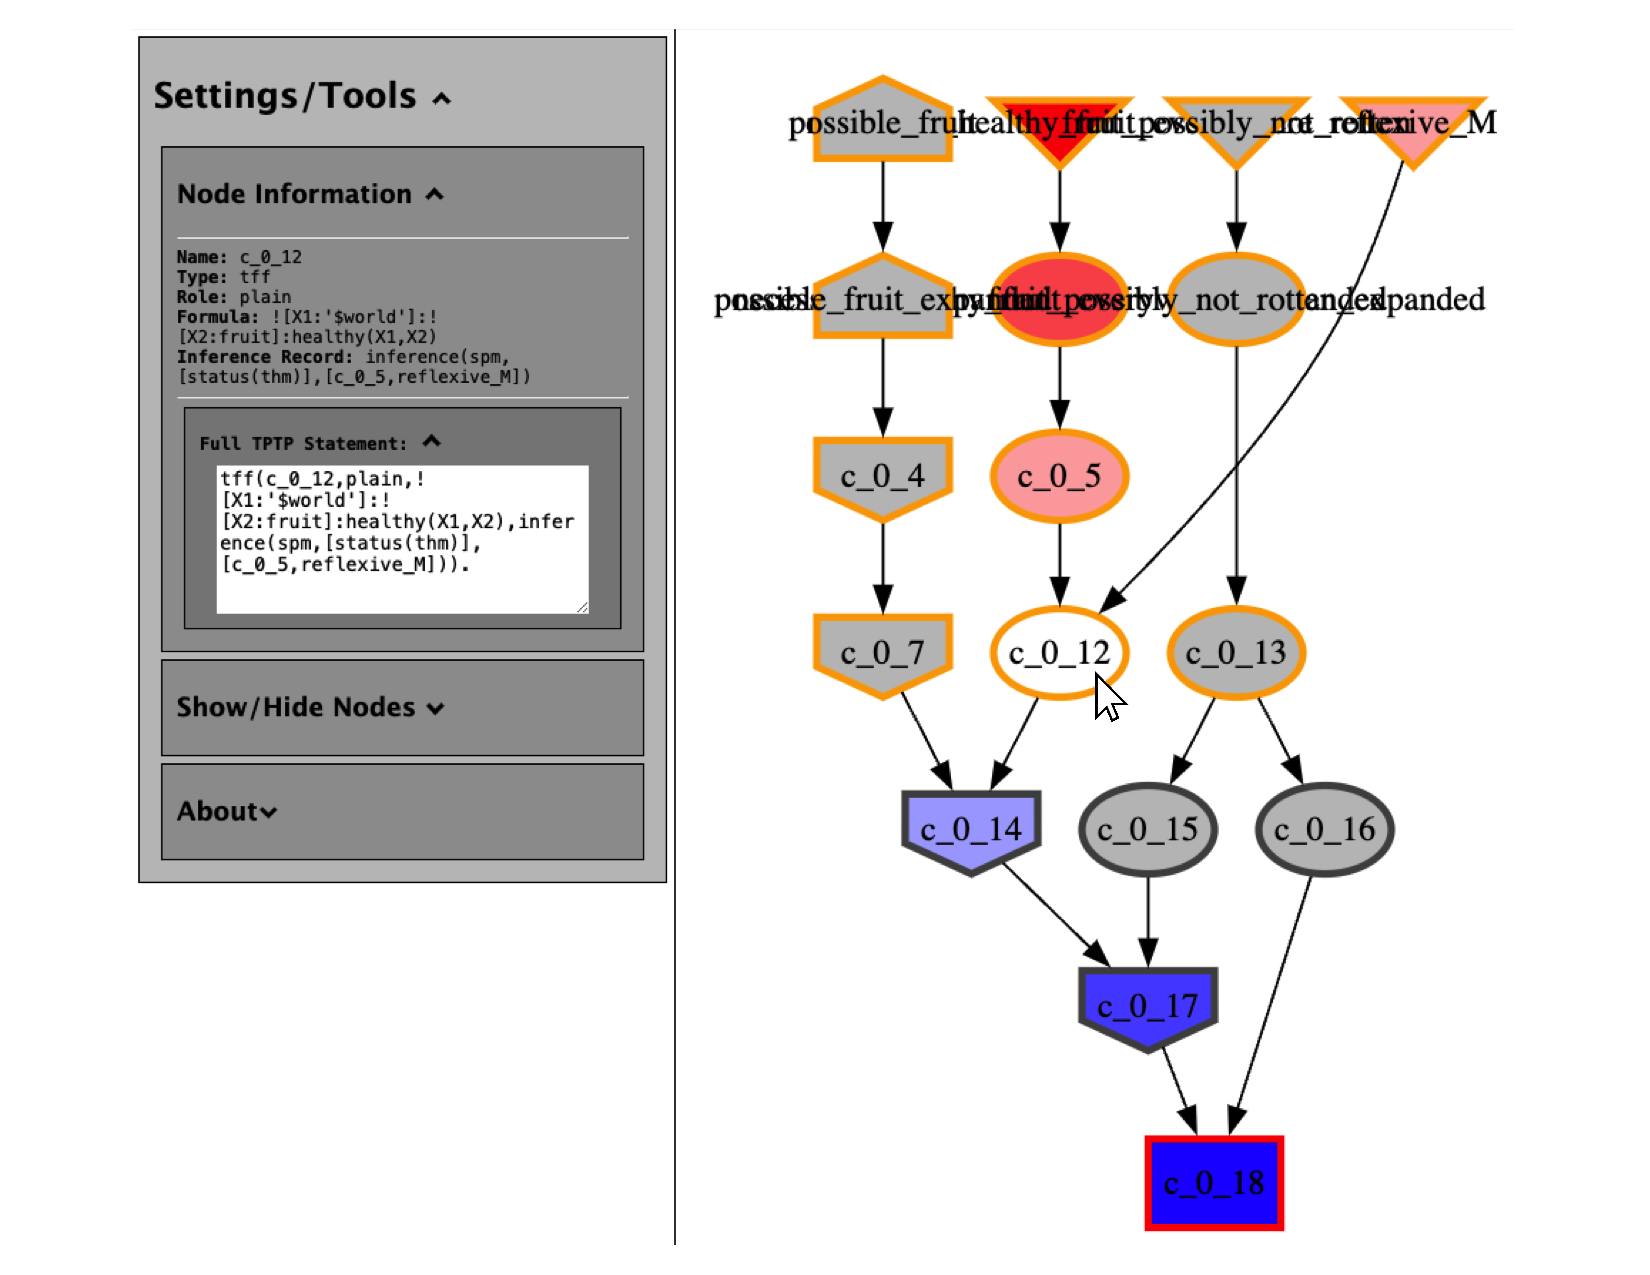
\includegraphics[width=0.75\textwidth]{NX0ProofIDV.pdf}
\caption{IDV view of the proof in Figure~\ref{NX0Proof}}
\label{NX0ProofIDV}
\end{figure}

The IIV Interactive Interpretation Viewer~\cite{SS+23-LPAR,MS23-Poster} can display the
Tarskian interpretation of a world in a Kripke model in TPTP format.
Figure~\ref{NX0InterpretationW1} shows the interpretation of world {\tt w1} in 
Figure~\ref{NX0Kripke}.
The pointer is hovering over the node {\tt d\_banana}.
The red {\tt \$o} ancestor indicates that {\tt rotten} has a boolean result type.
The blue {\tt \$true} descendant indicates that the interpretation of {\tt rotten} for the
domain element {\tt d\_banana} is {\em true}, and the blue {\tt \$o} descendant indicates that the
domain type is boolean.
A wrapper to view the worlds and accessibility relationship of a Kripke model is being developed,
which will be linked to IIV to view a chosen world's Tarskian interpretation.

\begin{figure}[htbp]
\centering
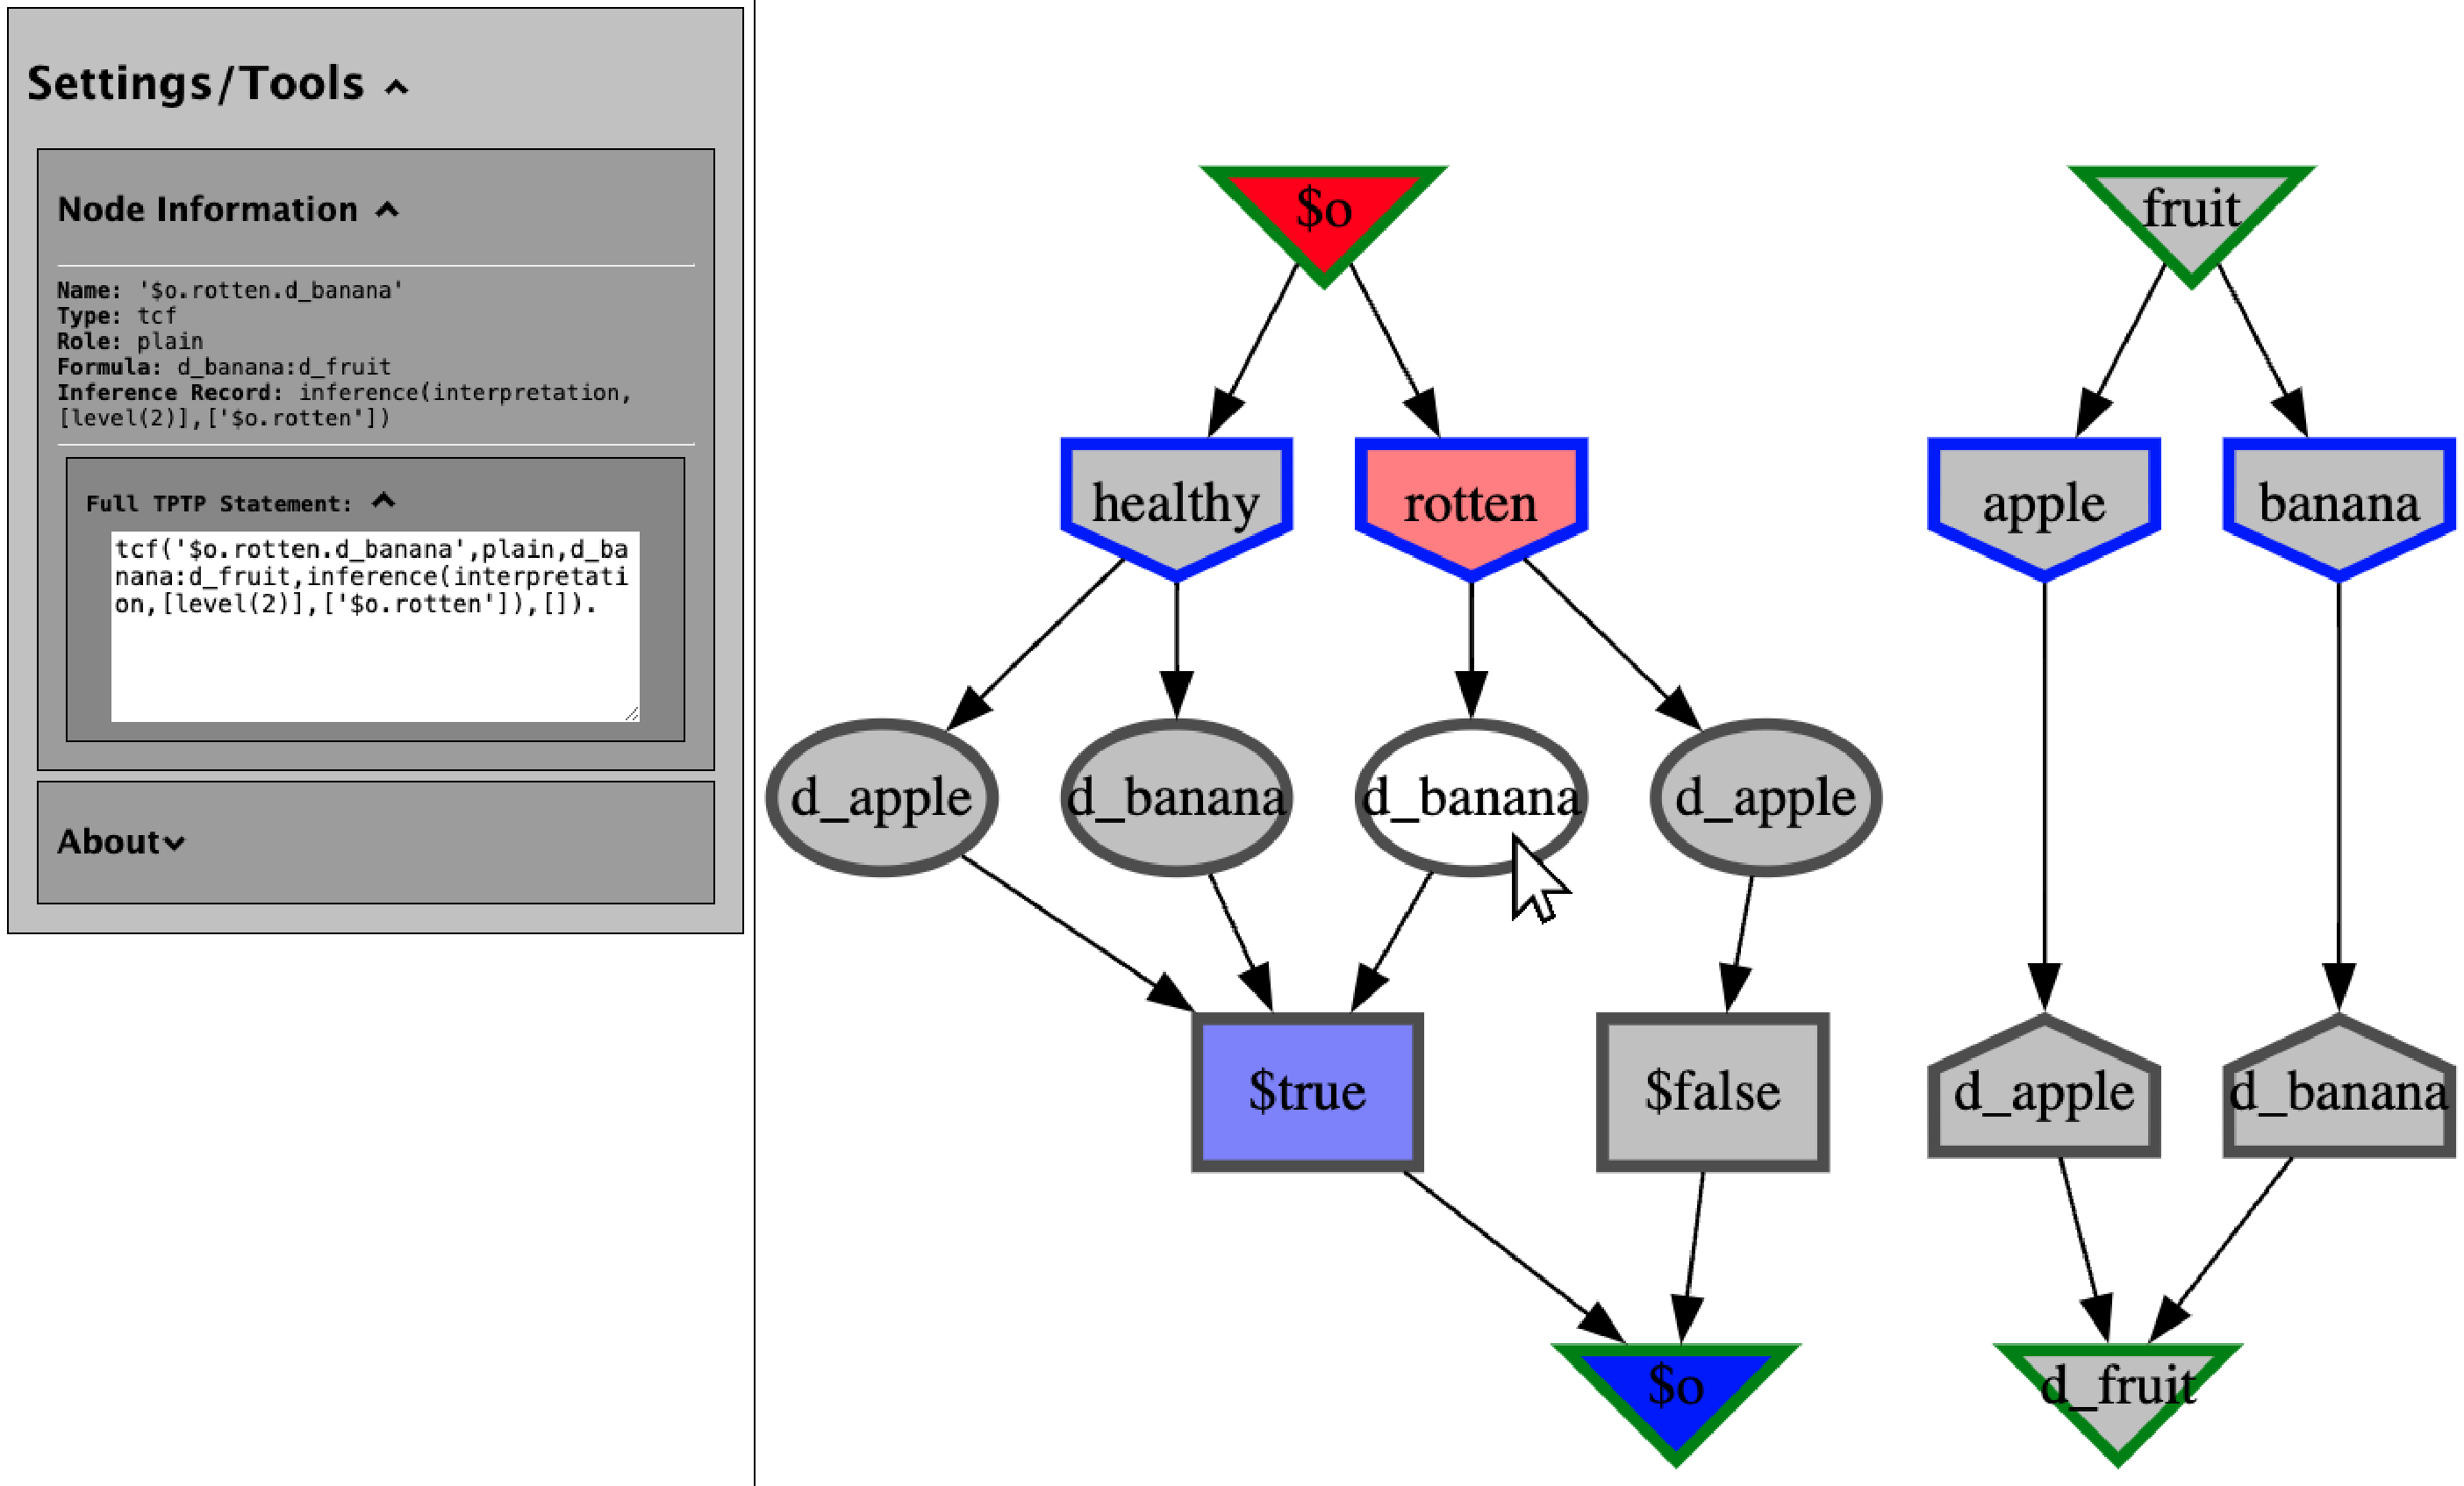
\includegraphics[width=0.75\textwidth]{NX0InterpretationW1.pdf}
\caption{IIV view of the interpretation of world {\tt w1} in Figure~\ref{NX0Kripke}}
\label{NX0InterpretationW1}
\end{figure}

IDV and IIV are available in SystemOnTSTP (see Section~\ref{Online}).

%--------------------------------------------------------------------------------------------------
\subsection{Online}
\label{Online}

The TPTP World has three online interfaces\footnote{%
\href{https://www.tptp.org/cgi-bin/SystemOnTPTP}{\tt www.tptp.org/cgi-bin/SystemOnTPTP}}
that provide access to ATP systems and tools:
SystemB4TPTP for preparing formulae (often problems) for systems and tools, SystemOnTPTP for 
submitting formulae to ATP systems, and SystemOnTSTP for processing solutions (often derivations
or models) from systems and tools \cite{Sut00-CADE-17,Sut07-CSR}.
SystemB4TPTP includes access to TPTP4X, the parsers, the KSP to TPTP translator, and NTFLET (see 
Section~\ref{Parsers}).
SystemOnTPTP includes the ATP systems KSP, nanoCoP-M, MleanCoP, and Leo-III.
SystemOnTSTP includes GDV, AGMV, IDV, IIV, and the {\tt InterpretByATP} for evaluating a formula
wrt a given interpretation (including Kripke interpretations) in TPTP format.

The TPTP2T tool for listing problems and solutions with specified syntactic and semantic 
characteristics is available in a separate interface\footnote{%
\href{https://tptp.org/cgi-bin/TPTP2T}{\tt tptp.org/cgi-bin/TPTP2T}}, e.g., it can be used to 
list NX0 problems that are theorems, contain equality, and are easy to prove.

%--------------------------------------------------------------------------------------------------
\section{Conclusion}
\label{Conclusion}

This paper describes the latest extension of the TPTP World, providing languages and
infrastructure for reasoning in non-classical logics.
That includes the NXF and NHF languages with non-classical connectives, and a new type of
of formula for specifying the logic to be used for reasoning.
The NXF and NHF languages are used for writing problems in non-classical logics, and the
TPTP format for writing Kripke interpretations is introduced.
ATP systems that can reason in non-classical logic, particularly those that can read 
problems written in TXF and THF, are listed, and tools for manipulating formulae written in 
NXF and NHF are described.
Altogether, this paper has described the keys steps towards releasing TPTP v9.0.0,
with modal logic problems.

Ongoing and future work includes~\ldots
\begin{packed_itemize}
\item Collecting lots more problems in non-classical logics.
\item Working with ATP system developers to upgrade their systems to natively read problems 
      written in NXF and NHF, and to produce proofs and models in NXF or NHF.
\item Optimizing the NTFLET embeddings to automatically recognize language fragments for which
      TXF embedding is possible.
\item Producing an interactive viewer for Kripke interpretations written in TPTP-format.
\item Standardizing the embedding of further specific non-classical logics in NXF/NHF (including
      choosing connective names, and allowed parameters of the logic specification).
\item A non-classical division of CASC.
\end{packed_itemize}

%--------------------------------------------------------------------------------------------------
%----LNCS \bibliographystyle{splncs04}
%----CEUR
% \bibliographystyle{splncs04}
\bibliography{Bibliography}
%--------------------------------------------------------------------------------------------------
\end{document}
